\section{Appendix}
\subsection{Attention structure.}\label{attn_structure}
A block-causal attention mask enforces temporal ordering while allowing information flow across modalities within each temporal block\cite{DreamZero}.
Temporal blocks group $b = 2$ tubelets (video) or $b = 2$ action steps.

\begin{figure}[h]
    \centering
    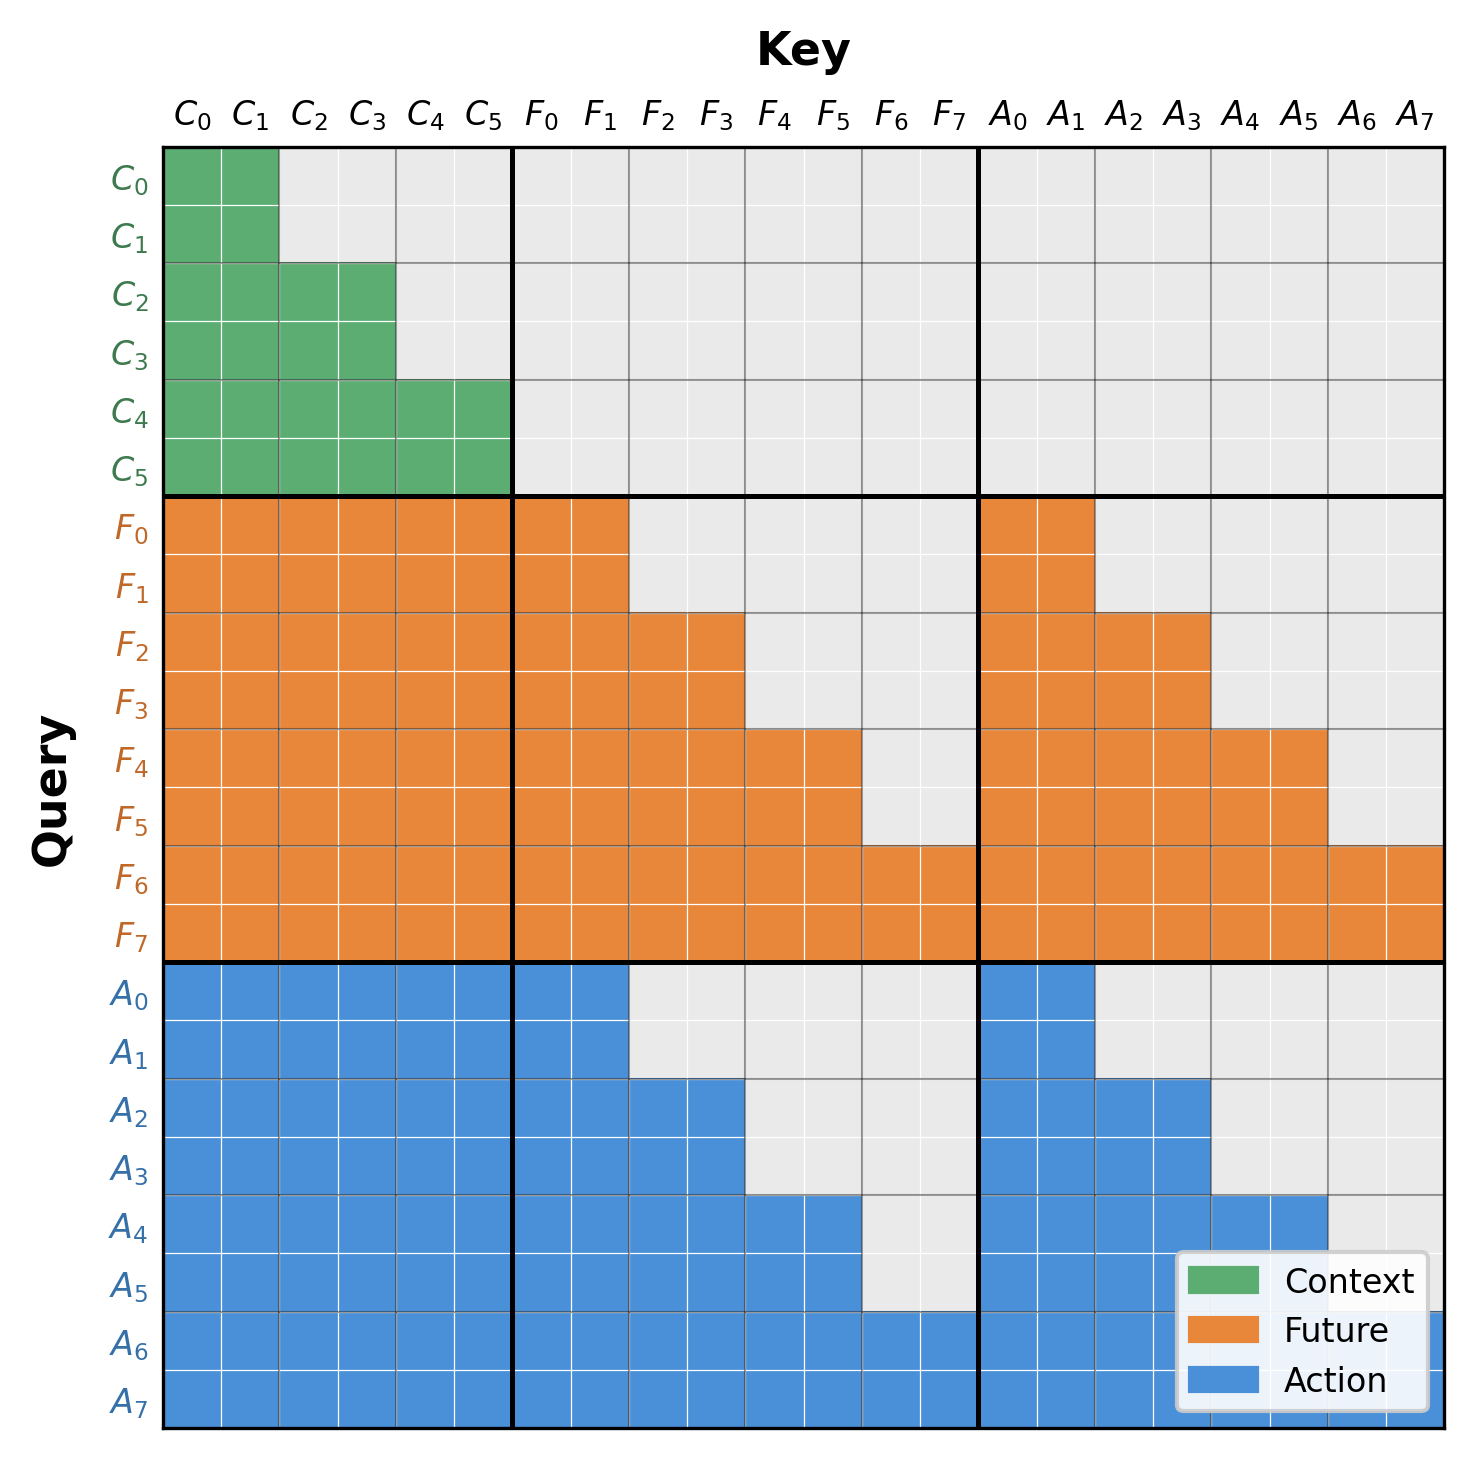
\includegraphics[width=0.6\columnwidth]{figures/generated/attn_mask.png}
    \caption{Block-causal attention mask. Colored cells indicate permitted attention. Context blocks are causally masked among themselves. Future and action blocks at temporal index $i$ attend to all context, all preceding blocks of both modalities up to $i$, enabling cross-modal information flow within each temporal step.}
    \label{fig:attn_mask}
\end{figure}

Specifically:
\begin{itemize}
    \item \textbf{Context block $i$}: attends to context blocks $0$ through $i$ (causal within context).
    \item \textbf{Future block $i$}: attends to all context, future blocks $0$ through $i$, and corresponding action blocks.
    \item \textbf{Action block $i$}: attends to all context, corresponding future blocks, and action blocks $0$ through $i$.
\end{itemize}
This cross-modal block alignment allows temporally co-occurring video and action predictions to inform each other during denoising.


